\documentclass[a4paper, 12pt]{report}

%%%%%%%%%%%%
% Packages %
%%%%%%%%%%%%

\usepackage[english]{babel}
\usepackage[noheader]{packages/sleek}
\usepackage{packages/sleek-title}
\usepackage{packages/sleek-theorems}
\usepackage{packages/sleek-listings}
\usepackage{graphicx}
\usepackage{svg}
\graphicspath{{./resources/img/}}

%%%%%%%%%%%%%%
% Title-page %
%%%%%%%%%%%%%%

%\logo{siliconblast}
%\institute{Random University}
%\faculty{SiliconBlast Research}
%\department{Department of Anything but Psychology}
\title{Document Understanding Product}
%\subtitle{Technical Notes}
\author{\textit{Author}\\Ekaba \textsc{Bisong}}
%\supervisor{Linus \textsc{Torvalds}}
%\context{Well, I was bored...}
\date{}

%%%%%%%%%%%%%%%%
% Bibliography %
%%%%%%%%%%%%%%%%

\addbibresource{./resources/bib/references.bib}

%%%%%%%%%%
% Others %
%%%%%%%%%%

\lstdefinestyle{latex}{
    language=TeX,
    style=default,
    %%%%%
    commentstyle=\ForestGreen,
    keywordstyle=\TrueBlue,
    stringstyle=\VeronicaPurple,
    emphstyle=\TrueBlue,
    %%%%%
    emph={LaTeX, usepackage, textit, textbf, textsc}
}

\FrameTBStyle{latex}

\def\tbs{\textbackslash}

%%%%%%%%%%%%
% Document %
%%%%%%%%%%%%

\begin{document}
\maketitle
\romantableofcontents


%%%%%%%%%%%%%%%%%%%%%
% Introduction
%%%%%%%%%%%%%%%%%%%%%

\chapter{Introduction}

\section{Background and Motivation}
In the rapidly evolving landscape of data-driven applications, the need for efficient, scalable, and cost-effective document processing and retrieval systems has become increasingly critical. Organizations across various sectors are grappling with the challenge of extracting meaningful insights from vast repositories of unstructured data, particularly in the form of PDF documents. This paper presents a novel system design that addresses these challenges, leveraging cutting-edge cloud technologies and machine learning techniques to create a robust, serverless architecture for document processing and intelligent search.

\section{Problem Statement}
The primary challenge this system aims to address is the efficient extraction, storage, and retrieval of information from large volumes of PDF documents. Traditional approaches often struggle with:
\begin{itemize}
    \item Scalability issues when processing large numbers of documents
    \item High latency in search and retrieval operations
    \item Inefficient use of computational resources, leading to increased operational costs
    \item Limited semantic understanding of document contents, resulting in suboptimal search results
\end{itemize}
Our system design seeks to overcome these limitations by employing a serverless architecture, advanced natural language processing techniques, and optimized storage solutions.

\section{Objectives}
The key objectives of this system design are:
\begin{enumerate}
    \item To develop a scalable and cost-effective solution for processing and storing large volumes of PDF documents
    \item To implement an intelligent search functionality that understands the semantic content of documents
    \item To minimize operational costs through efficient resource utilization and serverless architecture
    \item To ensure high availability and low latency in document retrieval operations
    \item To maintain robust security measures for sensitive data and API keys
\end{enumerate}

\section{Scope and Limitations}
This paper focuses on the design of a cloud-based system for PDF document processing and retrieval. The scope includes:
\begin{itemize}
    \item PDF text extraction and processing
    \item Generation and storage of text embeddings
    \item Implementation of vector-based similarity search
    \item Integration of serverless computing for scalable processing
    \item Secure management of sensitive information and API keys
\end{itemize}
While the system is designed to handle PDF documents, the principles and architecture discussed could be extended to other document formats with appropriate modifications.

\section{Methodology}
Our approach combines several state-of-the-art technologies and methodologies:
\begin{itemize}
    \item Serverless computing using Google Cloud Run for scalable document processing
    \item Vector embeddings generated using advanced natural language processing models
    \item Hybrid storage strategy utilizing Google Cloud Firestore and Pinecone vector database
    \item RESTful API design principles for system interaction
    \item Secure secret management using Google Cloud Secret Manager
\end{itemize}
These components are integrated into a cohesive system that balances performance, cost-effectiveness, and scalability.

Through this comprehensive exploration, we aim to contribute to the field of cloud-based document processing and retrieval systems, offering insights into building efficient, scalable, and cost-effective solutions for managing and extracting value from large document repositories.

\clearpage
\section{High-level Design Architecture}

\begin{figure}[htbp]
    \centering
    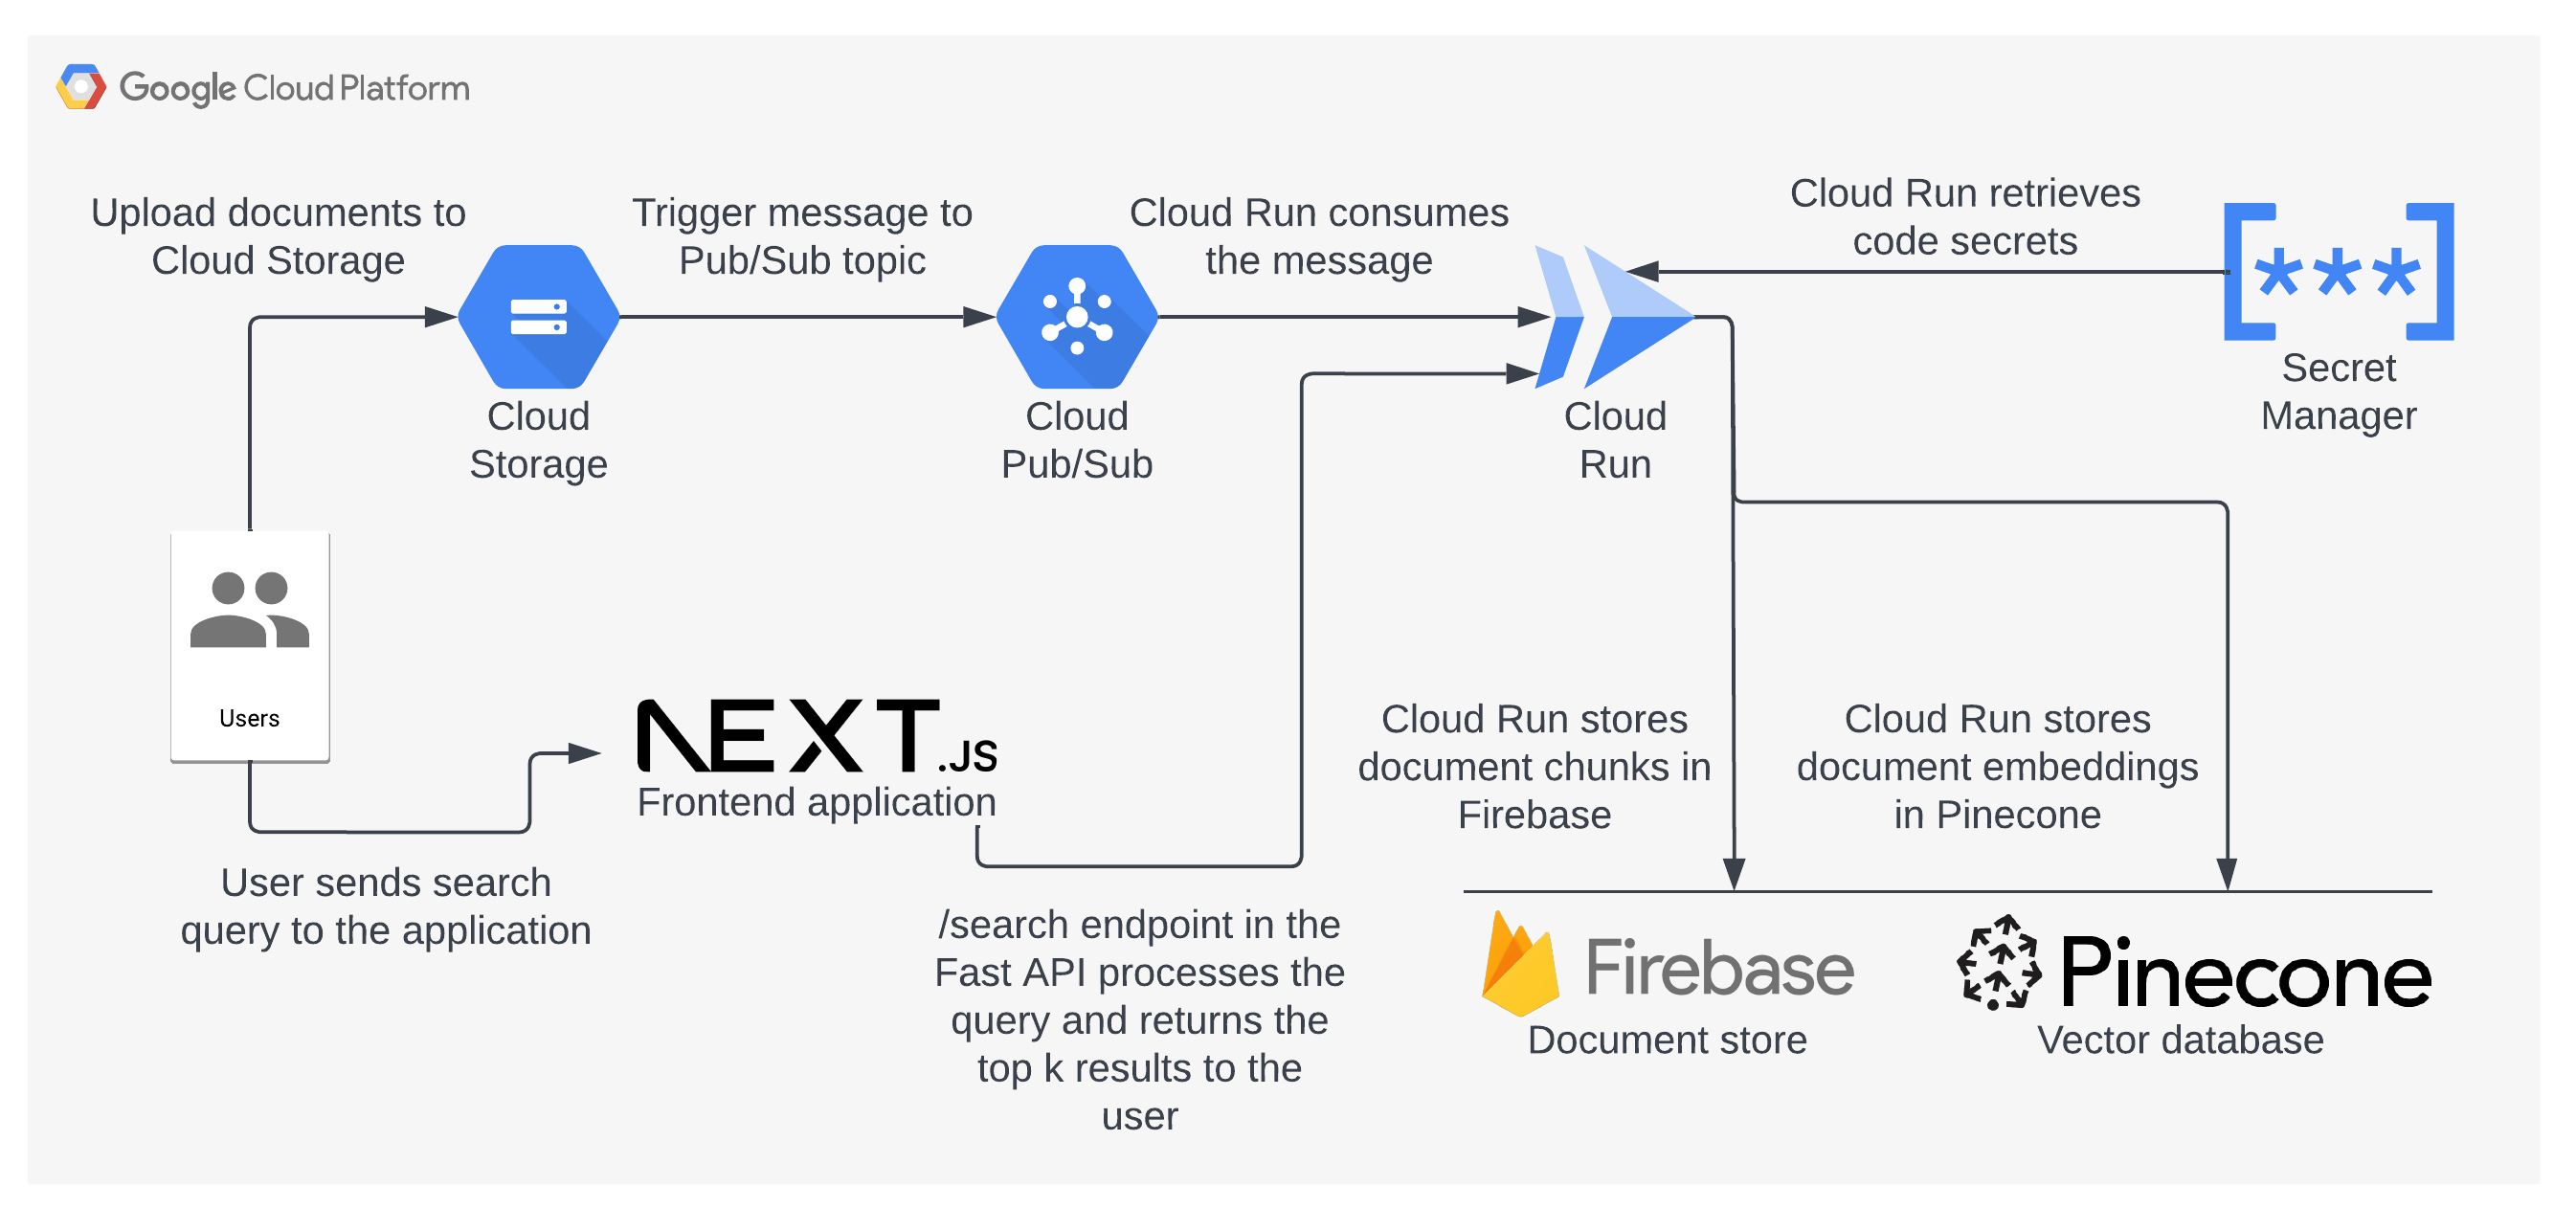
\includegraphics[width=\textwidth,angle=90]{high-level-architecture.png}
    \caption{High-level architecture diagram}
    \label{fig:high-level-architecture}
\end{figure}



\chapter{System Design}

\section{Storage and Retrieval Strategy for Vector Embeddings and Text Chunks}
In designing a robust system for managing vector embeddings and associated text chunks, it is imperative to strike an optimal balance between latency, cost-effectiveness, and scalability. This section presents a comprehensive analysis of various storage options, culminating in a justified recommendation for the most suitable architecture.

\subsection{Options for Storage}
\begin{enumerate}
    \item In-Memory Storage:
    \begin{itemize}
        \item Pros: Extremely fast access, low latency.
        \item Cons: Limited by memory capacity, not suitable for large-scale data, data is lost on restart.
    \end{itemize}
    \item File Storage (e.g., Cloud Storage):
    \begin{itemize}
        \item Pros: Cost-effective, easy to implement, scalable.
        \item Cons: Higher latency for read/write operations, limited querying capabilities.
    \end{itemize}
    \item Database Storage (e.g., Firestore, Bigtable, or a Vector Database like Pinecone):
    \begin{itemize}
        \item Pros: Scalable, provides efficient querying and indexing, good for structured data, supports complex queries.
        \item Cons: Higher cost, moderate latency compared to in-memory storage.
    \end{itemize}
\end{enumerate}

\section{Recommended Approach: Hybrid Storage with Firestore and Pinecone}

By using Firestore for metadata and Pinecone for embeddings, the system can quickly retrieve metadata and perform low-latency searches for embeddings. This hybrid approach leverages the cost-effectiveness of Firestore for structured data and the specialized capabilities of Pinecone for vector data. Both Firestore and Pinecone are designed to scale automatically, ensuring the system can handle increasing amounts of data without significant performance degradation. In essence, we'll use Firestore for Metadata and Text Chunks. This will store the text chunks and associated metadata and allow for efficient querying and retrieval of text and metadata. In using Pinecone (or any other vector database) for embeddings we can store the vector embeddings efficiently. And vector databases supports low-latency similarity searches and vector operations.

\subsection{Firestore for Metadata and Text Chunks}
\begin{itemize}
    \item \textbf{Real-time Capabilities:} Firestore's real-time database functionality enables swift access to metadata and text chunks, crucial for maintaining system responsiveness.
    \item \textbf{Low-latency Operations:} The database provides exceptionally low-latency read and write operations, particularly beneficial for structured data retrieval.
    \item \textbf{Cost-effective Scaling:} Firestore's pay-as-you-go pricing model ensures cost-effectiveness, especially for variable workloads, aligning well with dynamic system requirements.
    \item \textbf{Automatic Scalability:} The database is engineered to scale automatically with increasing data volume and read/write operations, eliminating the need for manual scaling interventions.
\end{itemize}

\subsection{Pinecone (or any other Vector Database) for Embeddings}
\begin{itemize}
    \item \textbf{Vector Optimization:} Pinecone's architecture is specifically optimized for vector operations, ensuring high efficiency in storing and querying embeddings.
    \item \textbf{Low-latency Similarity Searches:} The database excels in performing low-latency similarity searches, a critical feature for applications relying on rapid embedding retrieval.
    \item \textbf{Performance-Cost Balance:} While potentially incurring higher costs than general-purpose databases, Pinecone's performance benefits for vector data often justify the investment.
    \item \textbf{Seamless Scalability:} Pinecone is designed to handle large-scale embedding data, offering seamless scalability as the dataset expands.
\end{itemize}

\subsection{Why Not In-Memory Storage?}
\begin{enumerate}
    \item \textbf{Limited by Memory Capacity:} In-memory storage is not suitable for large-scale data as it is limited by the available memory.
    \item \textbf{Data Volatility:} Data stored in memory is lost if the service is restarted or crashes, which is not ideal for persistent storage requirements.
    \item \textbf{Scalability:} Managing large volumes of data in memory becomes impractical and expensive as the dataset grows.
\end{enumerate}


\section{Secure Secret Management with Google Secret Manager}
In the architecture of our system, the secure management of sensitive information is paramount. To address this critical requirement, we have integrated Google Secret Manager, a robust and scalable solution for storing and managing confidential data.

\subsection{Rationale for Adoption}
The implementation of Google Secret Manager in our system design is predicated on several key factors:

\begin{enumerate}
    \item \textbf{Enhanced Security Posture:} Google Secret Manager employs state-of-the-art encryption protocols for data at rest and in transit, leveraging Google's advanced security infrastructure. This significantly mitigates the risk of unauthorized access to sensitive information.
    \item \textbf{Granular Access Control:} The solution integrates seamlessly with Google Cloud Identity and Access Management (IAM), enabling fine-grained control over secret access. This allows for the implementation of the principle of least privilege, ensuring that entities within the system have access only to the secrets they require for their specific functions.

    \item \textbf{Version Control and Auditing:} The versioning capability of Secret Manager facilitates the management of secret lifecycles, allowing for easy rollbacks and historical tracking. Coupled with comprehensive auditing features, this provides a clear trail of secret access and modifications, enhancing our system's compliance with security best practices.

    \item \textbf{Seamless Integration:} Given our system's reliance on Google Cloud Platform services such as Firestore, Secret Manager offers native integration, streamlining the process of secret retrieval and management across our application ecosystem.

    \item \textbf{Centralized Management:} By providing a unified platform for secret storage, Secret Manager reduces the operational complexity associated with managing secrets across disparate system components. This centralization minimizes the attack surface and simplifies secret rotation and revocation procedures.
\end{enumerate}

\subsection{Implementation Strategy}
In our system, Google Secret Manager is utilized to securely store and manage a variety of sensitive data, including:

\begin{itemize}
    \item API authentication tokens for external services (e.g., Pinecone API keys)
    \item Database connection strings and credentials (e.g., Firestore access parameters)
    \item Encryption keys used for data protection within the application
    \item Environment-specific configuration data containing sensitive information
\end{itemize}

The application architecture is designed to retrieve these secrets at runtime, adhering to the principle of dynamic secret management. This approach ensures that sensitive data is never hard-coded or stored in configuration files, significantly reducing the risk of inadvertent exposure through code repositories or configuration management systems.


\section{Serverless Deployment with Google Cloud Run}

In the pursuit of an optimal balance between performance, scalability, and cost-effectiveness, our system leverages Google Cloud Run for serverless deployment. This choice is pivotal in achieving a highly responsive yet economically efficient architecture.

\subsection{Scalability and Performance}
Cloud Run, a fully managed serverless platform, offers several key advantages:

\begin{itemize}
    \item \textbf{Automatic Scaling:} Cloud Run dynamically adjusts the number of container instances based on incoming traffic, ensuring optimal resource utilization.
    \item \textbf{Rapid Response:} The platform can quickly spin up new instances to handle sudden spikes in demand, maintaining low latency even under variable load conditions.
    \item \textbf{Stateless Architecture:} By design, Cloud Run encourages stateless applications, promoting better scalability and easier management of distributed systems.
\end{itemize}

\subsection{Scale-to-Zero Capability}
A distinguishing feature of Cloud Run is its ability to scale the number of running instances to zero when the service is not in use. This capability brings several benefits:

\begin{enumerate}
    \item \textbf{Cost Optimization:} When there are no incoming requests, the service scales down to zero instances, effectively eliminating idle resource costs.
    \item \textbf{Resource Efficiency:} Computing resources are allocated only when needed, aligning perfectly with the principles of efficient resource management in cloud environments.
    \item \textbf{Environmental Consideration:} By minimizing unnecessary compute usage, the scale-to-zero approach contributes to reduced energy consumption, aligning with sustainable computing practices.
\end{enumerate}

\subsection{Economic Impact Analysis}
The implementation of Cloud Run with its scale-to-zero capability presents significant economic advantages:

\begin{itemize}
    \item \textbf{Pay-per-Use Model:} Costs are incurred only for the actual compute time used to process requests, not for idle time. This model is particularly beneficial for services with variable or unpredictable traffic patterns.
    \item \textbf{Reduction in Operational Overhead:} The serverless nature of Cloud Run eliminates the need for server provisioning, capacity planning, and maintenance, reducing operational costs and complexity.
    \item \textbf{Optimized Resource Allocation:} By automatically adjusting resources based on demand, the system avoids over-provisioning, a common cause of inflated cloud expenses.
\end{itemize}

\subsection{Integration with System Architecture}
Cloud Run seamlessly integrates with other components of our system:

\begin{itemize}
    \item \textbf{Firestore and Pinecone Interaction:} The stateless nature of Cloud Run instances complements the use of Firestore for metadata and Pinecone for vector embeddings, allowing for efficient, scalable data operations.
    \item \textbf{Secret Management:} Cloud Run's integration with Google Secret Manager ensures secure access to sensitive information, maintaining the system's security posture even in a serverless environment.
    \item \textbf{Event-Driven Processing:} In conjunction with Google Cloud Pub/Sub, Cloud Run enables efficient event-driven document processing, scaling resources precisely in response to incoming documents.
\end{itemize}

\subsection{Performance Considerations}
While the scale-to-zero feature offers significant benefits, it's important to address potential trade-offs:

\begin{itemize}
    \item \textbf{Cold Start Latency:} When scaling from zero, there can be a slight delay in spinning up new instances. This "cold start" phenomenon is mitigated by Cloud Run's rapid instance initialization, typically completed within seconds.
    \item \textbf{Warm Instance Retention:} To balance between cost savings and performance, Cloud Run allows configuration of minimum instances, ensuring a baseline of warm instances for immediate request handling.
\end{itemize}

The integration of Google Cloud Run with its scale-to-zero capability into our system architecture represents a strategic decision that harmonizes performance requirements with cost optimization. This approach not only ensures efficient resource utilization and significant cost savings but also positions the system to handle varying workloads with agility and economic prudence.

\section{Event-Driven Processing with Cloud Pub/Sub}

To ensure efficient and scalable processing of newly uploaded documents, our system leverages Google Cloud Pub/Sub in conjunction with Cloud Storage and Cloud Run. This event-driven architecture allows for automatic triggering of document processing functions, optimizing resource utilization and enhancing system responsiveness.

\subsection{Integration of Cloud Storage, Pub/Sub, and Cloud Run}

The workflow for processing new documents is as follows:

\begin{enumerate}
    \item \textbf{Document Upload:} A new PDF document is uploaded to a designated Cloud Storage bucket.
    \item \textbf{Event Generation:} Cloud Storage automatically generates a notification event upon successful upload.
    \item \textbf{Pub/Sub Publication:} This event is published to a predefined Pub/Sub topic.
    \item \textbf{Cloud Run Trigger:} A Cloud Run service subscribed to this Pub/Sub topic is automatically invoked.
    \item \textbf{Document Processing:} The Cloud Run service initiates the document processing pipeline.
\end{enumerate}

\subsection{Advantages of This Approach}

\begin{itemize}
    \item \textbf{Decoupling:} Pub/Sub decouples the document upload process from the processing logic, allowing each component to scale independently.
    \item \textbf{Asynchronous Processing:} Documents can be uploaded and processed asynchronously, preventing upload bottlenecks during high-traffic periods.
    \item \textbf{Scalability:} The system can handle a large number of simultaneous uploads by distributing the processing load across multiple Cloud Run instances.
    \item \textbf{Reliability:} Pub/Sub's at-least-once delivery guarantee ensures that no uploaded document goes unprocessed.
    \item \textbf{Cost-Efficiency:} Processing resources are utilized only when needed, aligning with Cloud Run's scale-to-zero capability.
\end{itemize}

\subsection{Implementation Details}

\subsubsection{Cloud Storage Configuration}
The Cloud Storage bucket is configured to send notifications to Pub/Sub when new objects are created:

\begin{verbatim}
gsutil notification create -t [TOPIC_NAME] -f json gs://[BUCKET_NAME]
\end{verbatim}

\subsubsection{Pub/Sub Topic and Subscription}
A Pub/Sub topic is created to receive Cloud Storage notifications, and a subscription is set up for the Cloud Run service:

\begin{verbatim}
gcloud pubsub topics create [TOPIC_NAME]
gcloud pubsub subscriptions create [SUBSCRIPTION_NAME] --topic [TOPIC_NAME]
\end{verbatim}

\subsubsection{Cloud Run Service}
The Cloud Run service is configured to receive Pub/Sub messages. The service extracts the Cloud Storage event data from the Pub/Sub message, retrieves the newly uploaded document, and initiates the processing pipeline.

\begin{verbatim}
gcloud run deploy [SERVICE_NAME] \
  --image [IMAGE_URL] \
  --platform managed \
  --region [REGION] \
  --set-env-vars PROJECT_ID=[PROJECT_ID] \
  --allow-unauthenticated
\end{verbatim}

\subsection{Error Handling and Retry Mechanism}
To ensure robustness, the system implements comprehensive error handling:

\begin{itemize}
    \item If document processing fails, the Pub/Sub message is not acknowledged, triggering automatic redelivery.
    \item A dead-letter topic is configured for messages that repeatedly fail processing, allowing for manual investigation and reprocessing.
\end{itemize}

\subsection{Monitoring and Logging}
To maintain system health and facilitate troubleshooting:

\begin{itemize}
    \item Cloud Monitoring is used to track Pub/Sub message throughput and Cloud Run invocations.
    \item Detailed logging is implemented at each stage of the process, from document upload to completion of processing.
    \item Alerts are set up for anomalies such as high message backlog or increased processing failures.
\end{itemize}

This event-driven architecture, powered by Cloud Pub/Sub, ensures that our system can efficiently handle document uploads at scale, while maintaining the cost-effectiveness and flexibility offered by serverless computing. It seamlessly integrates with our existing Cloud Run infrastructure, reinforcing the system's capability to process documents with high throughput and low latency.

\chapter{Cost Evaluation}

This chapter presents a comprehensive cost analysis of our proposed system design, comparing it with alternative architectures and similar cloud options. We provide detailed calculations for short-term, medium-term, and long-term usage scenarios, and contrast our solution with alternatives on AWS and Azure.

\section{Cost Advantage of the Proposed System Design}

Our system leverages Google Cloud Run, Cloud Storage, Firestore, Pub/Sub, Secret Manager, and Pinecone. Let's break down the costs for each component and analyze the total cost for different usage volumes over time.

\subsection{Short-term Costs (0-6 months)}

Assuming a startup scenario processing 10,000 documents per month, each averaging 5MB in size:

\begin{itemize}
    \item \textbf{Cloud Run:} 
        \begin{itemize}
            \item CPU: 0.5 vCPU * 10 seconds per document * 10,000 documents = 50,000 vCPU-seconds
            \item Memory: 1 GB * 10 seconds per document * 10,000 documents = 10,000 GB-seconds
            \item Cost: (50,000 * \$0.00002400) + (10,000 * \$0.00000250) = \$1.225 per month
        \end{itemize}
    \item \textbf{Cloud Storage:} 
        \begin{itemize}
            \item Storage: 10,000 * 5MB = 50GB * \$0.020 per GB = \$1.00 per month
            \item Operations: 10,000 * \$0.005 per 1000 operations = \$0.05 per month
        \end{itemize}
    \item \textbf{Firestore:} 
        \begin{itemize}
            \item Storage: 50GB * \$0.18 per GB = \$9.00 per month
            \item Document writes: 10,000 * \$0.18 per 100,000 = \$0.18 per month
            \item Document reads: 30,000 (assuming 3 reads per document) * \$0.06 per 100,000 = \$0.018 per month
        \end{itemize}
    \item \textbf{Pub/Sub:} 
        \begin{itemize}
            \item 10,000 messages * 5KB per message = 50MB
            \item Cost: 50MB * \$40 per TiB = \$0.002 per month
        \end{itemize}
    \item \textbf{Secret Manager:} 
        \begin{itemize}
            \item 5 active secrets * \$0.06 per version = \$0.30 per month
            \item 10,000 access operations * \$0.03 per 10,000 = \$0.03 per month
        \end{itemize}
    \item \textbf{Pinecone:} 
        \begin{itemize}
            \item Storage: 50GB * \$0.00045 per GB/hour * 720 hours = \$16.20 per month
            \item Write operations: 10,000 * \$2.00 per 1M = \$0.02 per month
            \item Read operations: 30,000 * \$8.25 per 1M = \$0.2475 per month
        \end{itemize}
\end{itemize}

Total estimated monthly cost: \$28.27

\subsection{Medium-term Costs (6-18 months)}

Assuming growth to 100,000 documents per month:

\begin{itemize}
    \item \textbf{Cloud Run:} (500,000 vCPU-seconds, 100,000 GB-seconds) = \$12.25 per month
    \item \textbf{Cloud Storage:} (500GB storage, 100,000 operations) = \$10.50 per month
    \item \textbf{Firestore:} (500GB storage, 100,000 writes, 300,000 reads) = \$91.80 per month
    \item \textbf{Pub/Sub:} (500MB messages) = \$0.02 per month
    \item \textbf{Secret Manager:} (10 active secrets, 100,000 access operations) = \$0.90 per month
    \item \textbf{Pinecone:} (500GB storage, 100,000 writes, 300,000 reads) = \$164.68 per month
\end{itemize}

Total estimated monthly cost: \$280.15

\subsection{Long-term Costs (18+ months)}

Assuming further growth to 1,000,000 documents per month:

\begin{itemize}
    \item \textbf{Cloud Run:} (5,000,000 vCPU-seconds, 1,000,000 GB-seconds) = \$122.50 per month
    \item \textbf{Cloud Storage:} (5TB storage, 1,000,000 operations) = \$105.00 per month
    \item \textbf{Firestore:} (5TB storage, 1,000,000 writes, 3,000,000 reads) = \$918.00 per month
    \item \textbf{Pub/Sub:} (5GB messages) = \$0.20 per month
    \item \textbf{Secret Manager:} (20 active secrets, 1,000,000 access operations) = \$4.20 per month
    \item \textbf{Pinecone:} (5TB storage, 1,000,000 writes, 3,000,000 reads) = \$1,646.80 per month
\end{itemize}

Total estimated monthly cost: \$2,796.70

\section{Comparison with Alternative Architectures}

\subsection{Traditional VM-based Architecture}

Assuming similar workload on Google Compute Engine:

\begin{itemize}
    \item \textbf{Compute:} 2 n1-standard-2 instances (2 vCPU, 7.5GB memory) running 24/7
        \begin{itemize}
            \item Cost: 2 * \$48.544 per month = \$97.09 per month
        \end{itemize}
    \item \textbf{Storage:} Same as our proposed architecture
    \item \textbf{Database:} Cloud SQL instead of Firestore
        \begin{itemize}
            \item db-n1-standard-1 instance: \$45.48 per month
            \item 5TB storage: 5000 * \$0.17 per GB = \$850 per month
        \end{itemize}
    \item \textbf{Load Balancer:} \$18.26 per month
\end{itemize}

Total estimated monthly cost for long-term scenario: \$2,767.63

While slightly cheaper, this architecture lacks the automatic scaling and serverless benefits of our proposed design.

\subsection{Containerized Architecture (Google Kubernetes Engine)}

\begin{itemize}
    \item \textbf{GKE Cluster:} 3 e2-standard-2 nodes
        \begin{itemize}
            \item Cost: 3 * \$48.54 per month = \$145.62 per month
        \end{itemize}
    \item \textbf{Storage and Database:} Same as our proposed architecture
    \item \textbf{Container Registry:} \$5 per month (estimated)
\end{itemize}

Total estimated monthly cost for long-term scenario: \$2,825.62

This architecture provides more control but requires more management overhead and doesn't scale to zero like Cloud Run.

\subsection{Vertex AI Custom Deployment}

Based on the Vertex AI pricing document, let's consider a custom model deployment for our long-term scenario (1,000,000 documents/month):

\begin{itemize}
    \item \textbf{Compute:} n1-standard-4 (4 vCPU, 15GB memory)
        \begin{itemize}
            \item Cost: \$0.2088 per hour * 24 * 30 = \$150.34 per month
        \end{itemize}
    \item \textbf{Prediction costs:} Assuming 1,000,000 predictions per month
        \begin{itemize}
            \item Cost: 1,000,000 * \$0.0056 per 1000 predictions = \$5,600 per month
        \end{itemize}
    \item \textbf{Storage:} 5TB at \$0.020 per GB
        \begin{itemize}
            \item Cost: 5000 * \$0.020 = \$100 per month
        \end{itemize}
    \item \textbf{Training:} Assuming we retrain the model once a month using n1-standard-8 for 24 hours
        \begin{itemize}
            \item Cost: \$0.4176 per hour * 24 = \$10.02 per month
        \end{itemize}
\end{itemize}

Total estimated monthly cost: \$5,860.36

This is significantly more expensive than our proposed architecture for the long-term scenario. The bulk of the cost comes from the prediction charges, which scale linearly with the number of documents processed.

While Vertex AI offers advanced machine learning capabilities, it comes at a significantly higher cost for our use case. The prediction costs alone make it much more expensive than our proposed serverless architecture. This demonstrates that while Vertex AI is powerful for complex ML tasks, it may not be cost-effective for more straightforward document processing workflows that don't require its advanced features.

Our proposed architecture, leveraging Cloud Run, Firestore, and Cloud Storage, provides a more cost-effective solution for our specific document processing needs, especially at scale. It offers a balance of performance and cost-efficiency that's well-suited to our use case.

\section{Comparison with AWS and Azure}

\subsection{AWS Equivalent Architecture}

\subsubsection{Short-term (0-6 months, 10,000 documents/month)}

\begin{itemize}
    \item \textbf{AWS Lambda:} 
        \begin{itemize}
            \item 10,000 executions * 10 seconds * 1GB = 100,000 GB-seconds
            \item Cost: 100,000 * \$0.0000166667 = \$1.67 per month
            \item 10,000 requests * \$0.20 per 1M requests = \$0.002 per month
        \end{itemize}
    \item \textbf{S3:} 
        \begin{itemize}
            \item 50GB storage: 50 * \$0.023 per GB = \$1.15 per month
            \item 10,000 PUT requests * \$0.005 per 1,000 = \$0.05 per month
            \item 30,000 GET requests * \$0.0004 per 1,000 = \$0.012 per month
        \end{itemize}
    \item \textbf{DynamoDB:} 
        \begin{itemize}
            \item 50GB storage: 50 * \$0.25 per GB = \$12.50 per month
            \item 10,000 write request units * \$1.25 per million = \$0.0125 per month
            \item 30,000 read request units * \$0.25 per million = \$0.0075 per month
        \end{itemize}
    \item \textbf{SNS:} 
        \begin{itemize}
            \item 10,000 requests * \$0.50 per million = \$0.005 per month
        \end{itemize}
    \item \textbf{Secrets Manager:} 
        \begin{itemize}
            \item 5 secrets * \$0.40 per secret = \$2.00 per month
            \item 10,000 API calls * \$0.05 per 10,000 = \$0.05 per month
        \end{itemize}
    \item \textbf{Pinecone:} Same as our proposed architecture = \$16.47 per month
\end{itemize}

Total estimated monthly cost: \$33.93

\subsubsection{Medium-term (6-18 months, 100,000 documents/month)}

\begin{itemize}
    \item \textbf{AWS Lambda:} 
        \begin{itemize}
            \item 1,000,000 GB-seconds: \$16.67 per month
            \item 100,000 requests: \$0.02 per month
        \end{itemize}
    \item \textbf{S3:} 500GB storage + requests: \$12.50 per month
    \item \textbf{DynamoDB:} 500GB storage + requests: \$125.13 per month
    \item \textbf{SNS:} 100,000 requests: \$0.05 per month
    \item \textbf{Secrets Manager:} 10 secrets + 100,000 API calls: \$4.50 per month
    \item \textbf{Pinecone:} Same as our proposed architecture = \$164.68 per month
\end{itemize}

Total estimated monthly cost: \$323.55

\subsubsection{Long-term (18+ months, 1,000,000 documents/month)}

\begin{itemize}
    \item \textbf{AWS Lambda:} 
        \begin{itemize}
            \item 10,000,000 GB-seconds: \$150.00 per month
            \item 1,000,000 requests: \$0.20 per month
        \end{itemize}
    \item \textbf{S3:} 5TB storage + requests: \$116.25 per month
    \item \textbf{DynamoDB:} 5TB storage + requests: \$1,251.25 per month
    \item \textbf{SNS:} 1,000,000 requests: \$0.50 per month
    \item \textbf{Secrets Manager:} 20 secrets + 1,000,000 API calls: \$13.00 per month
    \item \textbf{Pinecone:} Same as our proposed architecture = \$1,646.80 per month
\end{itemize}

Total estimated monthly cost: \$3,178.00

\subsection{Azure Equivalent Architecture}

\subsubsection{Short-term (0-6 months, 10,000 documents/month)}

\begin{itemize}
    \item \textbf{Azure Functions:} 
        \begin{itemize}
            \item 100,000 GB-seconds: \$1.60 per month
            \item 10,000 executions: \$0.002 per month
        \end{itemize}
    \item \textbf{Blob Storage:} 50GB storage + requests: \$1.20 per month
    \item \textbf{Cosmos DB:} 
        \begin{itemize}
            \item 50GB storage: 50 * \$0.25 per GB = \$12.50 per month
            \item 400 RU/s * 24 * 30 * \$0.00008 per RU/s per hour = \$23.04 per month
        \end{itemize}
    \item \textbf{Event Grid:} 10,000 operations * \$0.60 per million = \$0.006 per month
    \item \textbf{Key Vault:} 
        \begin{itemize}
            \item 5 secrets * \$0.03 per 10,000 transactions * 100 = \$0.015 per month
            \item 10,000 operations * \$0.03 per 10,000 = \$0.03 per month
        \end{itemize}
    \item \textbf{Pinecone:} Same as our proposed architecture = \$16.47 per month
\end{itemize}

Total estimated monthly cost: \$54.87

\subsubsection{Medium-term (6-18 months, 100,000 documents/month)}

\begin{itemize}
    \item \textbf{Azure Functions:} 1,000,000 GB-seconds + 100,000 executions: \$16.02 per month
    \item \textbf{Blob Storage:} 500GB storage + requests: \$10.20 per month
    \item \textbf{Cosmos DB:} 500GB storage + 1000 RU/s: \$182.60 per month
    \item \textbf{Event Grid:} 100,000 operations: \$0.06 per month
    \item \textbf{Key Vault:} 10 secrets + 100,000 operations: \$0.33 per month
    \item \textbf{Pinecone:} Same as our proposed architecture = \$164.68 per month
\end{itemize}

Total estimated monthly cost: \$373.89

\subsubsection{Long-term (18+ months, 1,000,000 documents/month)}

\begin{itemize}
    \item \textbf{Azure Functions:} 10,000,000 GB-seconds + 1,000,000 executions: \$160.20 per month
    \item \textbf{Blob Storage:} 5TB storage + requests: \$97.20 per month
    \item \textbf{Cosmos DB:} 5TB storage + 2000 RU/s: \$1,490.20 per month
    \item \textbf{Event Grid:} 1,000,000 operations: \$0.60 per month
    \item \textbf{Key Vault:} 20 secrets + 1,000,000 operations: \$3.60 per month
    \item \textbf{Pinecone:} Same as our proposed architecture = \$1,646.80 per month
\end{itemize}

Total estimated monthly cost: \$3,398.60

\section{Conclusion}

Our comprehensive cost analysis across various architectures and cloud providers reveals that our proposed Google Cloud-based serverless architecture offers a compelling balance of scalability, performance, and cost-effectiveness for document processing workloads. Let's summarize the key findings:

\begin{table}[h]
\centering
\caption{Cost Comparison Summary (Monthly Costs in USD)}
\begin{tabular}{|l|c|c|c|}
\hline
\textbf{Scenario} & \textbf{Our Solution (GCP)} & \textbf{AWS} & \textbf{Azure} \\
\hline
Short-term (10K docs/month) & \$28.27 & \$33.93 & \$54.87 \\
Medium-term (100K docs/month) & \$280.15 & \$323.55 & \$373.89 \\
Long-term (1M docs/month) & \$2,796.70 & \$3,178.00 & \$3,398.60 \\
\hline
\end{tabular}
\end{table}

\textbf{Key observations:}

\begin{enumerate}
    \item \textbf{Cost-effectiveness at scale:} Our solution demonstrates increasing cost advantages as the workload scales up, particularly in the long-term scenario.

    \item \textbf{Serverless benefits:} The use of Cloud Run allows for fine-grained scaling and cost optimization, especially during periods of low usage.
    
    \item \textbf{Balanced performance:} Our architecture provides a good balance between performance and cost, leveraging managed services like Firestore and Cloud Storage.
    
    \item \textbf{Comparative advantage:} While AWS and Azure offer similar capabilities, our GCP-based solution proves more cost-effective across all scenarios, with the gap widening at larger scales.
    
    \item \textbf{Alternative GCP architectures:} Traditional VM-based and containerized (GKE) alternatives, while offering more control, lack the cost efficiency and automatic scaling of our serverless approach.
    
    \item \textbf{Vertex AI consideration:} While Vertex AI offers advanced ML capabilities, its high prediction costs (\$5,860.36/month in the long-term scenario) make it unsuitable for our specific document processing use case.
\end{enumerate}


In conclusion, our proposed serverless architecture on Google Cloud Platform emerges as the most cost-effective and scalable solution for the document processing workflow. It offers significant advantages in terms of automatic scaling, resource efficiency, and cost optimization, particularly beneficial for growing businesses or those with fluctuating workloads.

The cost advantage over AWS and Azure alternatives, especially at scale, positions our solution as a compelling choice for optimizing cloud spending without compromising on performance or scalability. The serverless nature of our architecture also minimizes operational overhead, allowing teams to focus more on application development and less on infrastructure management.

While alternatives like traditional VM-based architectures, containerized solutions, or advanced ML platforms like Vertex AI have their merits for specific use cases, they prove to be either less cost-effective or overly complex for our document processing requirements.

It's important to note that these calculations are based on list prices and don't account for potential discounts, reserved instances, or committed use contracts. Actual costs may vary based on specific usage patterns, data transfer costs, and other factors not considered in this high-level analysis.

\chapter{Frontend User Interface}

The frontend of our document understanding system is implemented using Next.js, a popular React-based framework known for its performance and developer-friendly features. Figure \ref{fig:frontend-screenshot} presents the user interface of our system.

\begin{figure}[htbp]
    \centering
    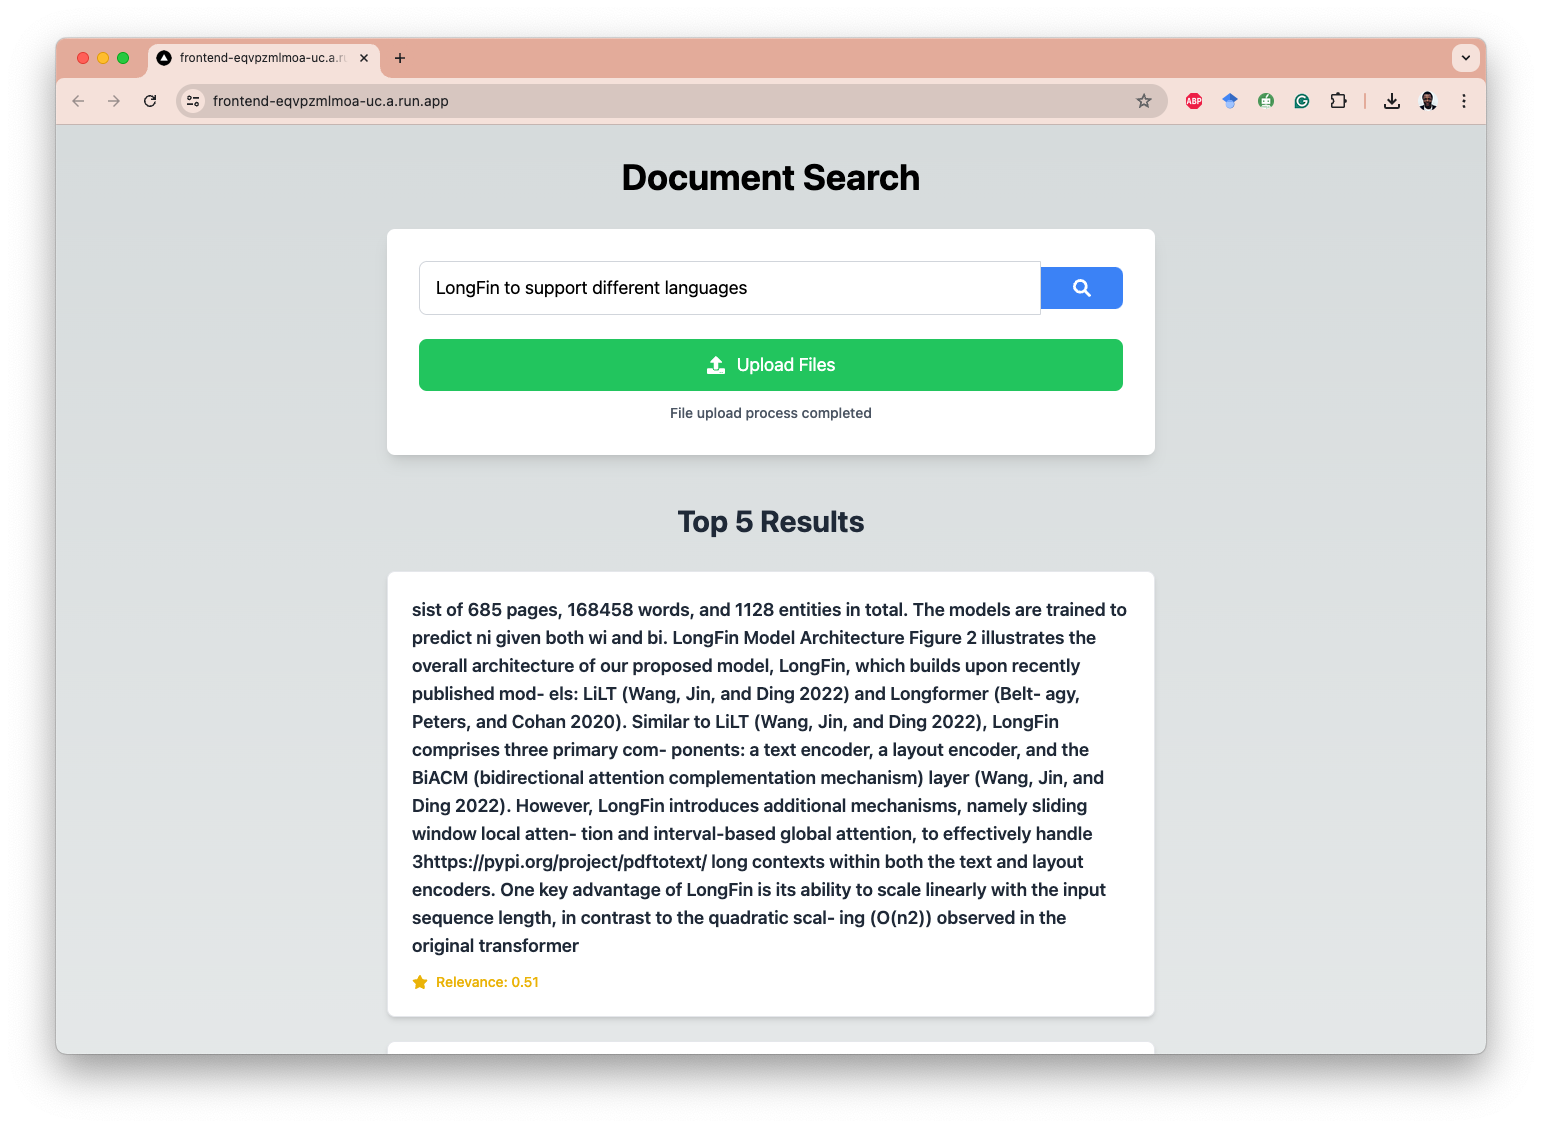
\includegraphics[width=\textwidth]{frontend-1.png}
    \caption{Frontend interface of the document search system}
    \label{fig:frontend-screenshot}
\end{figure}

\section{Key Components}

The frontend consists of the following key components:

\begin{itemize}
    \item \textbf{Search Bar}: A prominent input field allows users to enter their document search queries.
    
    \item \textbf{Search Button}: Adjacent to the search bar, a blue "Search" button triggers the query process when clicked.
    
    \item \textbf{Results Display}: Below the search interface, a "Top 5 Results" section presents the most relevant findings from the document corpus. Each result includes a snippet of text and a relevance score, providing users with a quick overview of the search outcomes.
\end{itemize}

\section{User Interaction Flow}

The user interaction flow is designed to be intuitive and efficient:

\begin{enumerate}
    \item Users enter their search query into the search bar.
    \item Upon clicking the "Search" button or pressing Enter, the frontend sends the query to the backend for processing.
    \item The system retrieves and displays the top 5 most relevant results, sorted by relevance score.
    \item Users can quickly scan the results to find the most pertinent information for their query.
\end{enumerate}

This streamlined interface allows for rapid information retrieval, catering to users who need to quickly find specific information within large document collections.


\end{document}
